% ----------------------------------------------------
% PR Integration
% ----------------------------------------------------
\documentclass[class=report,11pt,crop=false]{standalone}
% Page geometry
\usepackage[a4paper,margin=25mm,top=25mm,bottom=25mm]{geometry}

% Font choice
\usepackage{lmodern}

% Use IEEE bibliography style
\bibliographystyle{IEEEtran}

% Line spacing
\usepackage{setspace}
\setstretch{1.20}

% Ensure UTF8 encoding
\usepackage[utf8]{inputenc}

% Language standard (not too important)
\usepackage[english]{babel}

% Skip a line in between paragraphs
\usepackage{parskip}

% For the creation of dummy text
\usepackage{blindtext}

% Math
\usepackage{amsmath}

% Header & Footer stuff
\usepackage{fancyhdr}
\pagestyle{fancy}
\fancyhead{}
\fancyhead[R]{\nouppercase{\rightmark}}
\fancyfoot{}
\fancyfoot[C]{\thepage}
\renewcommand{\headrulewidth}{0.0pt}
\renewcommand{\footrulewidth}{0.0pt}
\setlength{\headheight}{13.6pt}

% Page geometry
\usepackage[a4paper,top=25mm,bottom=25mm]{geometry}

% Epigraphs
\usepackage{epigraph}
\setlength\epigraphrule{0pt}

% Hyperlinks & References
\usepackage{hyperref}
\hypersetup{
    colorlinks=true,
    linkcolor=blue,
    filecolor=blue,      
    urlcolor=blue,
    citecolor=blue,
}
\urlstyle{same}

% Automatically correct front-side quotes
\usepackage[autostyle=false, style=american]{csquotes}
\MakeOuterQuote{"}

% Graphics
\usepackage{graphicx}
\graphicspath{{Images/}{../Images/}}

% Colour
\usepackage{color}
\usepackage[usenames,dvipsnames]{xcolor}

% SI units
\usepackage{siunitx}

% Microtype goodness
\usepackage{microtype}

% Listings
\usepackage{listings}
\definecolor{backgroundColour}{RGB}{250,250,250}
\definecolor{commentColour}{RGB}{73, 175, 102}
\definecolor{identifierColour}{RGB}{196, 19, 66}
\definecolor{stringColour}{RGB}{252, 156, 30}
\definecolor{keywordColour}{RGB}{50, 38, 224}
\definecolor{lineNumbersColour}{RGB}{127,127,127}
\lstset{ 
  language=Matlab,
  captionpos=b,
  backgroundcolor=\color{backgroundColour},
  basicstyle=\footnotesize,        % the size of the fonts that are used for the code
  breakatwhitespace=false,         % sets if automatic breaks should only happen at whitespace
  breaklines=true,                 % sets automatic line breaking
  postbreak=\mbox{\textcolor{red}{$\hookrightarrow$}\space},
  commentstyle=\color{commentColour},    % comment style
  identifierstyle=\color{identifierColour},
  stringstyle=\color{stringColour},
   keywordstyle=\color{keywordColour},       % keyword style
  %escapeinside={\%*}{*)},          % if you want to add LaTeX within your code
  extendedchars=true,              % lets you use non-ASCII characters; for 8-bits encodings only, does not work with UTF-8
  frame=single,	                   % adds a frame around the code
  keepspaces=true,                 % keeps spaces in text, useful for keeping indentation of code (possibly needs columns=flexible)
  morekeywords={*,...},            % if you want to add more keywords to the set
  numbers=left,                    % where to put the line-numbers; possible values are (none, left, right)
  numbersep=5pt,                   % how far the line-numbers are from the code
  numberstyle=\tiny\color{lineNumbersColour}, % the style that is used for the line-numbers
  rulecolor=\color{black},         % if not set, the frame-color may be changed on line-breaks within not-black text (e.g. comments (green here))
  showspaces=false,                % show spaces everywhere adding particular underscores; it overrides 'showstringspaces'
  showstringspaces=false,          % underline spaces within strings only
  showtabs=false,                  % show tabs within strings adding particular underscores
  stepnumber=1,                    % the step between two line-numbers. If it's 1, each line will be numbered
  tabsize=2,	                   % sets default tabsize to 2 spaces
  %title=\lstname                   % show the filename of files included with \lstinputlisting; also try caption instead of title
}

% Caption stuff
\usepackage{caption}
\usepackage{subcaption}

\makenoidxglossaries

\newacronym{radar}{RADAR}{Radio Detection and Ranging}
\newacronym{dab}{DAB}{Digital Audio Broadcasting}
\newacronym{fm}{FM}{Frequency Modulation}
\newacronym{am}{AM}{Amplitude Modulation}
\newacronym{fdm}{FDM}{Frequency Division Multiplexing}
\newacronym{ofdm}{OFDM}{Orthogonal Frequency Division Multiplexing}
\newacronym{cofdm}{COFDM}{Coded Orthogonal Frequency Division Multiplexing}
\newacronym{dvbt2}{DVB–T2}{Digital Video Broadcasting — Second Generation Terrestrial}
\newacronym{em}{EM}{electromagnetic}
\newacronym{icasa}{ICASA}{Independent Communications Authority of South Africa}
\newacronym{ioo}{IOO}{Illuminators of Opportunity}
\newacronym{pr}{PR}{Passive Radar}
\newacronym{qpsk}{QPSK}{Differential Quadrature Phase-Shift Keying}
\newacronym{dqpsk}{DQPSK}{Differential Quadrature Phase-Shift Keying}
\newacronym{etsi}{ETSI}{European Telecommunications Standards Institute}
\newacronym{psk}{PSK}{Phase Shift Keying}
\newacronym{ask}{ASK}{Amplitude-Shift Keying}
\newacronym{fsk}{FSK}{Frequency-Shift Keying}
\newacronym{iq}{IQ}{In-phase and Quadrature}
\newacronym{prs}{PRS}{Phase Reference Symbol}
\newacronym{dft}{DFT}{Discrete Fourier Transform}
\newacronym{fft}{FFT}{Fast Fourier Transform}
\begin{document}
% ----------------------------------------------------
\chapter{Passive Radar Integration \label{ch:pr-integration}}
\epigraph{Oh, to see without my eyes.}%
    {\emph{---Sufjan Stevens}}
% ----------------------------------------------------

\section{Overview}
This brief chapter serves to provide a rudimentary insight into the context for which the \gls{dab} processing chain was designed: integration into a \gls{pr} system. The scope of this project did not facilitate a thorough analysis into such integration, and the details surrounding its performance, accuracy, and efficiency were not considered in any way. Instead, the work done for this chapter was purely illustrative, included to demonstrate the bigger picture to the reader, in a way that omits dense mathematical analysis.

\section{System Description}
A conventional, bistatic \gls{pr} system requires two signals for its operation: a reference signal, and a surveillance signal. The former is the signal that arrives via the direct-path, from the uncooperative transmitter to system's receiver. The latter is the signal that comes from the scene, as a recording of the scatterings and reflections of the \gls{em} energy. However, when a \emph{digitally}-modulated signal is used---one which has an open and accessible standard, such as the \gls{etsi}'s \gls{dab} standard---the reference data can be generated using the surveillance data. This trick enables the system to use only one antenna for operations, which is advantageous in various ways. Several authors have discussed such systems in further detail, such as in~\cite{Barott2014},~\cite{Searle2015}, and~\cite{Fang2018}.

The aim of this project was to design the functionality for converting surveillance data into reference data for a given \gls{dab} signal. This was done via the demodulation of the received signal, and then the remodulation thereof, thereby producing a "perfect" copy of the received signal. This perfect copy (used as reference data), together with the original recorded signal (used as surveillance data), could be provided to a standard \gls{pr} algorithm for further processing and analysis. A block diagram depicting the larger \gls{pr}~system's set-up is provided in Figure~\ref{fig:BD_pr-integration}.

\begin{figure}[htbp]
    \centering
    \captionsetup{type=figure}
    \def\svgwidth{\linewidth}
    {\setstretch{0.7} % Line spacing
    \scriptsize
    \input{../Images/BD_pr-integration.pdf_tex}}
    \caption{Block diagram showing how the \texttt{demodulate} and \texttt{remodulate} blocks fit into a larger \glsentrytext{pr} system.}
    \label{fig:BD_pr-integration}
\end{figure}

One can see in the figure how the \texttt{pre-process}, \texttt{demodulate}, and \texttt{remodulate} blocks fit into the context of a \gls{pr} system. Note, however, that the \texttt{pre-process} block would likely be markedly different in such a system, compared to the one designed in this project. For example, the data from the baseband receiver would likely be streamed, rather than read from a file, as it was done here. The other two blocks may also be slightly different when implemented in a real system, but their fundamental routines would remain the same. As shown, the reference and surveillance data from the \gls{dab} processing chain must always be synchronised before being used in the \gls{pr} processing chain.

For the sake of brevity, details of the \texttt{baseband receiver} and \texttt{synchronise} blocks are not given here. Moreover, specifics of the \texttt{passive radar processing} chain are similarly omitted.

\section{Illustration}
A common output that is plotted for a particular \gls{pr} situation is the \gls{ard} map, which shows the two-dimensional cross-correlation of the reference and surveillance data over a finite integration period. This plot can be used to identify targets from a scene. To illustrate the use of a \gls{dab} signal in a \gls{pr} chain, and what an \gls{ard} map might look like in such a situation, a simple simulation was performed.

The simulation was based off an arbitrary, perfect \gls{dab} signal, \(x[n]\). To simulate an object in a scene, a delayed and doppler-shifted version of this signal was created, called \(y[n]\), with a bistatic range of~\(d_0\) and doppler shift of \(f_0\). A normally-distributed random noise signal was also defined, \(\eta[n]\). The surveillance signal was then defined as the sum of these signals, with the latter two scaled by constants~\(K\) and~\(\sigma\) respectively, to control their relative weightings in the simulation:
\begin{equation}
    s[n] = x[n] + K \cdot y[n] + \sigma \cdot \eta[n]
\end{equation}
Ideally, by passing the surveillance signal through the demodulation-remodulation processing chain, the original \gls{dab} signal, \(x[n]\), would have been recovered. However, depending on the echo and noise signals added, some bit-errors may have arisen in the processed signal. Nonetheless, this reconstructed signal was used as the reference signal:
\begin{equation}
    r[n] = \mathrm{Remod}\bigg\{\:\mathrm{Demod}\Big\{\; s[n]\;\Big\}\:\bigg\}
\end{equation}

These two signals, the surveillance and reference, were passed into a provided \gls{pr} processing chain, with an \gls{ard} map as the output. A variety of situations were simulated, with different values chosen for each parameter. Note that the parameter \(\sigma\) controlled the \gls{snr}. Four of the simulation results are shown in Figure~\ref{fig:integration-simulation-all}, with red circles superimposed to highlight the simulated object's location in each.

\begin{figure}[htbp]
    \centering
    \captionsetup{type=figure}
    \begin{subfigure}[t]{0.49\textwidth}
        \centering
        \captionsetup{type=figure}
        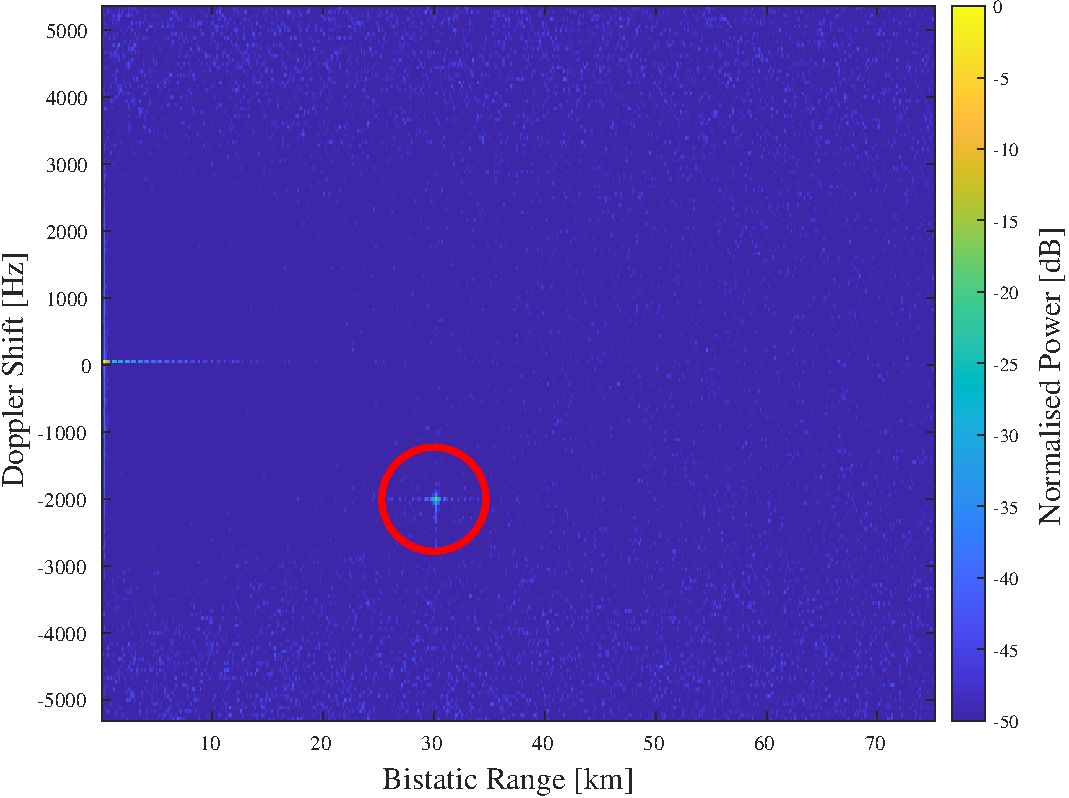
\includegraphics[width=\linewidth]{plots/integration-30km-2000Hz-K20-noise0.pdf}
        \caption{\(d_0 = 30\si{\kilo\metre}\); \(f_0 = -2\si{\kilo\hertz}\); \(K = 0.2\); \(\textrm{SNR} = 0\si{\deci\bel}\)}
        \label{fig:integration-simulation-1}
    \end{subfigure}%
    ~~
    \begin{subfigure}[t]{0.49\textwidth}
        \centering
        \captionsetup{type=figure}
        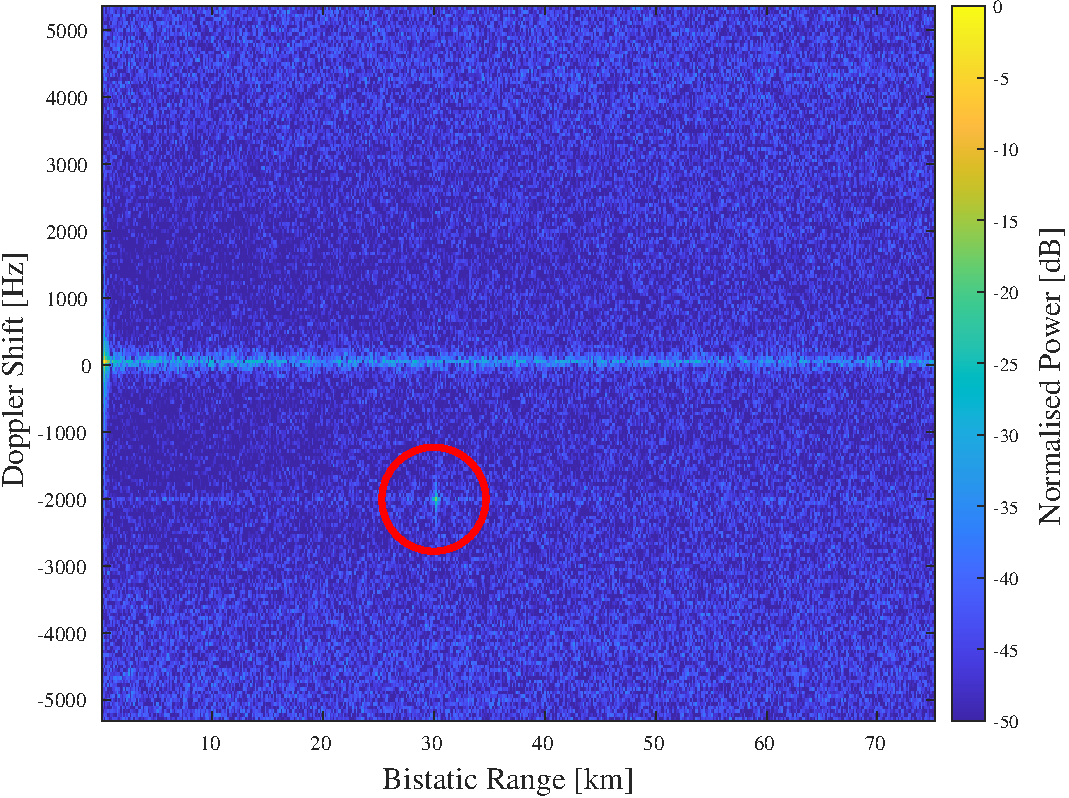
\includegraphics[width=\linewidth]{plots/integration-30km-2000Hz-K20-noise10dB.pdf}
        \caption{\(d_0 = 30\si{\kilo\metre}\); \(f_0 = -2\si{\kilo\hertz}\); \(K = 0.2\); \(\textrm{SNR} = 10\si{\deci\bel}\)}
        \label{fig:integration-simulation-2}
    \end{subfigure}%
    \\
    \begin{subfigure}[t]{0.49\textwidth}
        \centering
        \captionsetup{type=figure}
        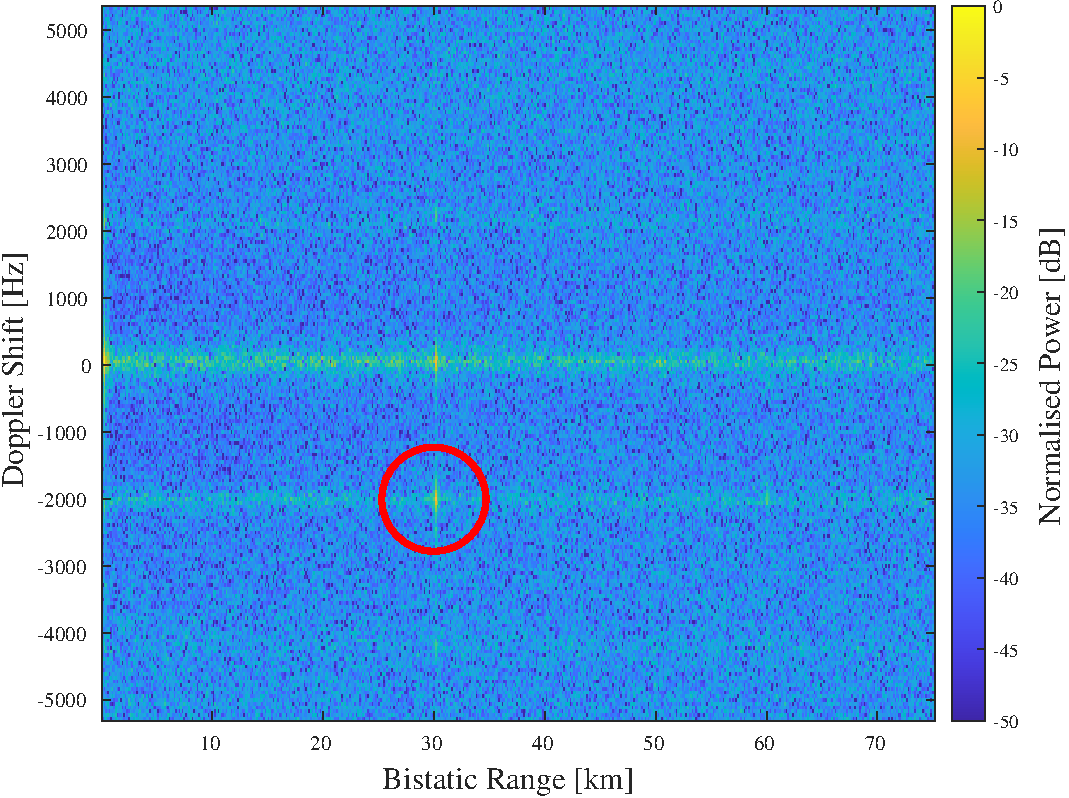
\includegraphics[width=\linewidth]{plots/integration-30km-2000Hz-K80-noise0.pdf}
        \caption{\(d_0 = 30\si{\kilo\metre}\); \(f_0 = -2\si{\kilo\hertz}\); \(K = 0.8\); \(\textrm{SNR} = 0\si{\deci\bel}\)}
        \label{fig:integration-simulation-3}
    \end{subfigure}%
    ~~
    \begin{subfigure}[t]{0.49\textwidth}
        \centering
        \captionsetup{type=figure}
        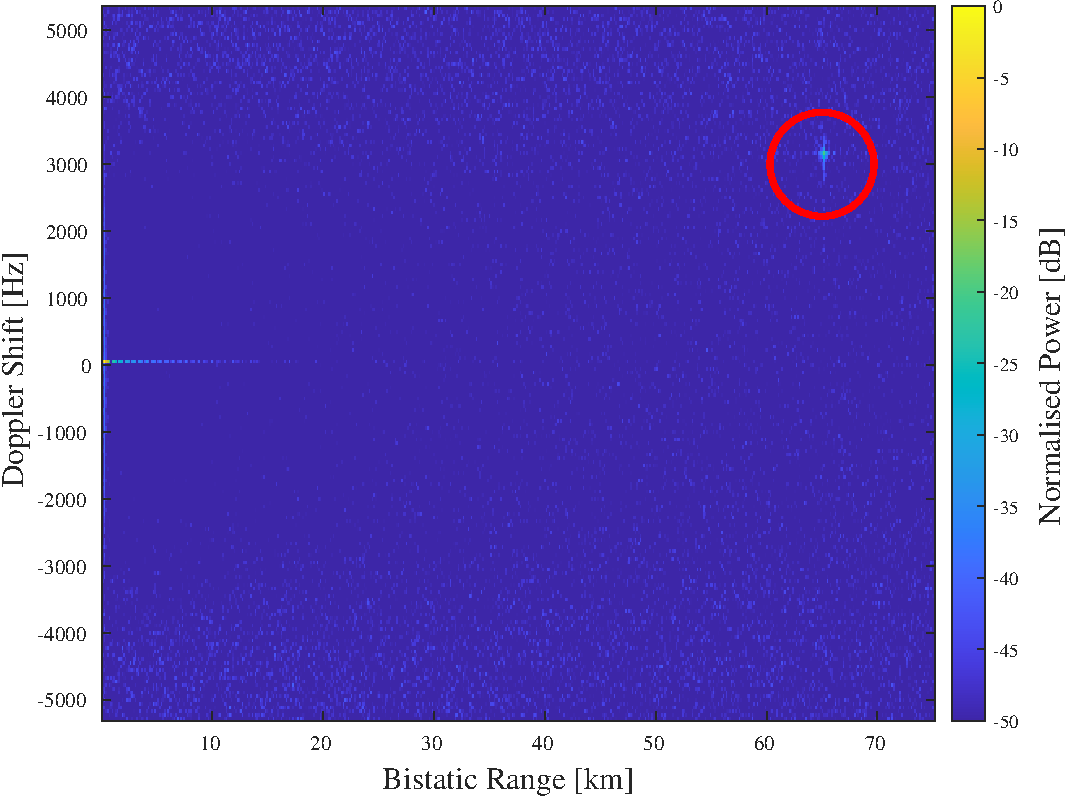
\includegraphics[width=\linewidth]{plots/integration-65km-3000Hz-K20-noise0.pdf}
        \caption{\(d_0 = 65\si{\kilo\metre}\); \(f_0 = +3\si{\kilo\hertz}\); \(K = 0.2\); \(\textrm{SNR} = 0\si{\deci\bel}\)}
        \label{fig:integration-simulation-4}
    \end{subfigure}%
    \caption{Results from four of the simulations of a \glsentrytext{dab} signal in a \glsentrytext{pr} processing chain.}
    \label{fig:integration-simulation-all}
\end{figure}

This short chapter has simply illustrated how the \gls{dab} processing blocks fit into a larger \gls{pr} chain, and how an output thereof might appear. There is clearly scope for further investigation, both in simulation and in real-world testing.

% ----------------------------------------------------
\ifstandalone
\bibliography{../Bibliography/References.bib}
\printnoidxglossary[type=\acronymtype,nonumberlist]
\fi
\end{document}
% ----------------------------------------------------